\documentclass[a4paper, 12pt]{article}

\usepackage{graphicx}

\begin{document}
	\author{Alex Aalbertsberg (s1008129)}	
	\title{APiE Assignment 1: Complexity, Debugging, Optimizing}
	\maketitle
	\newpage
	\part*{1}
	- Changed filename to listofprimes.m to correctly reflect the function name.\\
	- Line 20: (primes = 2:N) moved to a conditional statement with the 
	condition N $<$ 2. If this condition is not met (therefore N $>$= 2), 
	we create an array with numbers 2 to N.\\
	- Line 23: Changed != to \textasciitilde= (\textasciitilde= is not equals in MATLAB).\\
	- Line 26: Added semicolon to the end of the line to signify statement end.\\
	- In order to allow the function to return the result array, 
	added the name of the variable (primes) to the function signature.\\
	- The return statement is not required.\\\\
	END OF SOLVING M-LINT ERRORS.\\
	---------------------------------------------------------------------------\\
	Running the program as it is after fixing M-LINT errors/warnings,
	for example through listofprimes(10) will return "N must be a scalar".
	Since 10 is obviously a scalar value, we need to modify the condition that
	checks for it. We can use the isscalar(N) function to perform the check 
	properly. This function will return 0 if N is not a scalar, and 1 if it is.
	After this, the program will run without errors.
	However, the output is still incorrect. listofprimes(10) returns the values
	2, 3, 4, 6 and 8, whereas the primes between 2 and 10 should be 2, 3, 5 and 
	7. First of all, the if-statement within the for loop is checking the wrong
	indices for the value 0. Because we are not adding the number 1 to the 
	vector, we should check for k-1. Then, we can change the value in the
	vector that should be set to 0 to the following: primes(k+(k-1):k:N) = 0;
	This will solve the issues and provide the correct list of primes. The correct code can be found in the enclosed file listofprimes.m.
	\newpage
	\part*{2}
	1. \\
	The code for this question can be found in the file matrix\_product\_complexity.m.	
	The question talks about square matrices, therefore their dimensions must 
	both be n x n. Under normal circumstances, with a x b and b x c matrices, 
	the order would be $O(a*b*c)$. The reason for this is because the loops in the algorithm loop once from 1 to a, once from 1 to b and once from 1 to c. In this case, because we are talking about 
	square matrices (n x n), the order of the multiplication equals $O(n^3)$.\\\\
	2. \\
	Dependence on n seems to be about $n^3$ (see Figure 1). n can be about 4500 such 
	that it can still be computed within 10 seconds.\\
	\begin{figure}[!ht]
		\centering
		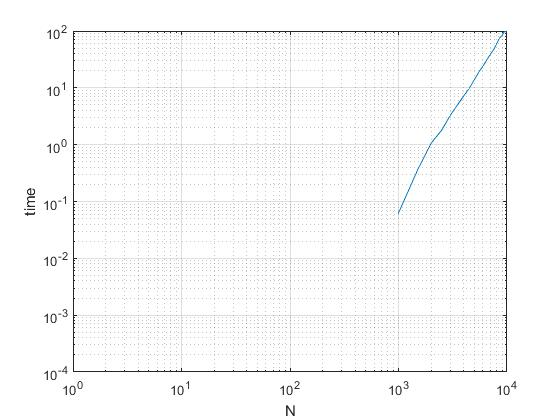
\includegraphics[width=\textwidth]{2}
		\caption{Log-log plot of the timing of Algorithm 1}
	\end{figure}	
	\newpage
	\part*{3}
	The difference becomes noticeable at high values for the length of the 
	vectors. Lines 9 $(d(k) = sqrt(x(k)^2 + y(k)^2 + z(k)^2))$ and 10 (end) take up most of the computation time.
	I have made some modifications to the function as a whole. Firstly, I have 
	concatenated the three arguments for the function into one matrix. 
	Secondly, I have inserted a check to see if the matrix consists of the 
	dimensions 3xN.
	After that, we square each element of the matrix and calculate the total 
	sum of each row. This single column vector of sums can then be used to 
	calculate each of the distances to the origin.
	The resulting code is enclosed as minDistance.m.
	\newpage
	\part*{4}
	The algorithm seems to maintain a factorial complexity (n!) in terms of 
	both time and memory. The reason behind this is that all permutations 
	have to be both computed (requires n! computations) and stored (requires n! 
	vectors in memory).
	
	Since we have a factorial complexity algorithm on our hands, I will compute
	the time required to perform the algorithm for values N of 1 through 10. At 
	the maximum value of this range, this already constitutes a set of nearly 
	4 million unique permutations! There is a bit of strange behavior in the 
	graph; this is possibly a result of the fact that the algorithm is cached 
	after running the first time. This would cause the speed of the algorithm to 
	seemingly speed up after the first execution. (See figure 2.)
	\begin{figure}[!ht]
		\centering
		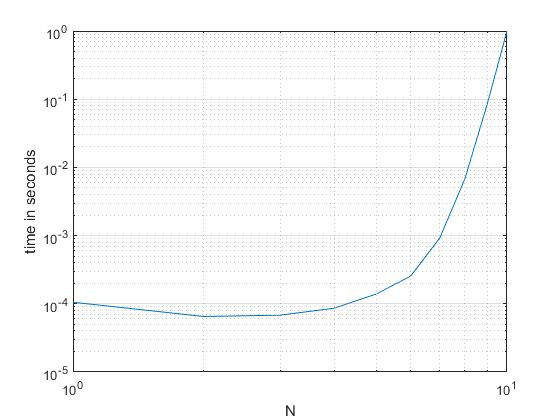
\includegraphics[width=\textwidth]{4}
		\caption{Log-log plot of the timing of the perms algorithm.}
	\end{figure}
	
\end{document}